\subsubsection{UCS 1 - Accesso al server}%kite level

\begin{itemize}
\item \textbf{Attori primari:} Amministratore non autenticato
\item \textbf{Precondizione:} L'amministratore non è autenticato.
\item \textbf{Postcondizione:} L'amministratore viene autenticato all'interno del sistema tramite \glo{autenticazione} [UCS 1.1].
\item \textbf{Scenario principale:} L'amministratore non autenticato può accedere, tramite l'\glo{autenticazione} [UCS 1.1], al server. 
%\item \textbf{Estensioni:}
\end{itemize}

\subsubsection{UCS 1.1 - Autenticazione al Server}

\begin{figure}[h]
    \centering
    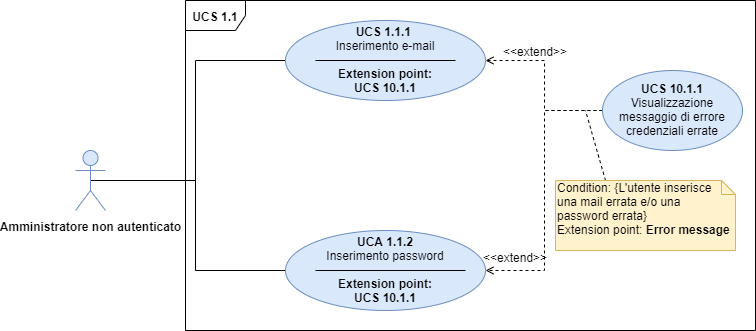
\includegraphics[scale=0.6]{Sezioni/UseCase/Immagini/UCS1.1.png}
    \caption{UCS 1.1 - \glo{Autenticazione} al Server}
\end{figure}

\begin{itemize}
\item \textbf{Attori primari:} Amministratore non autenticato
\item \textbf{Precondizione:} L'amministratore non è autenticato.
\item \textbf{Postcondizione:} L'amministratore è stato autenticato e può avere accesso alle funzionalità offerte dal sistema.
\item \textbf{Scenario principale:} Amministratore non identificato inserisce e-mail e la password per autenticarsi al server.
\item \textbf{Scenario alternativo 1:} L'amministratore tenta di accede con delle credenziali errate [UCS 10.1.1].
\item \textbf{Scenario alternativo 2:} Qualora l'amministratore non dovesse ricordarsi la password può selezionare la funzionalità "password dimenticata" per reimpostarla [UCS 1.3].
\item \textbf{Flusso di eventi:}
    \begin{enumerate}
        \item Inserimento e-mail [UCS 1.1.1];
        \item Inserimento password [UCS 1.1.2];
        \item L'amministratore seleziona la funzionalità di accesso.
    \end{enumerate}
    \item \textbf{Inclusioni:}
	\begin{itemize}		
		\item UCS 1.1.1 - Inserimento e-mail;
		\item UCS 1.1.2 - Inserimento password.
	\end{itemize}
    \item \textbf{Estensioni:}
    \begin{itemize}
		\item UCS 10.1.1 - Visualizzazione messaggio di errore credenziali errate;
		\item UCS 1.3 - Password dimenticata.
	\end{itemize}
\end{itemize}

\subsubsection{UCS 1.1.1 - Inserimento e-mail}%sea level
\begin{itemize}
\item \textbf{Attori primari:} Amministratore non autenticato
%\item \textbf{Attori secondari:}%opzionale
\item \textbf{Precondizione:} L'amministratore non è autenticato.
\item \textbf{Postcondizione:} L'amministratore ha inserito la propria e-mail.
\item \textbf{Scenario principale:} Inserimento dell'e-mail per l'autenticazione al Server.
\end{itemize}

\subsubsection{UCS 1.1.2 - Inserimento password}%sea level
\begin{itemize}
\item \textbf{Attori primari:} Amministratore non autenticato
%\item \textbf{Attori secondari:}%opzionale
\item \textbf{Precondizione:} L'amministratore non è autenticato.
\item \textbf{Postcondizione:} L'amministratore ha inserito la propria password.
\item \textbf{Scenario principale:} Inserimento della password per l'autenticazione al Server.
\end{itemize}

\begin{figure}[h]
	\centering
	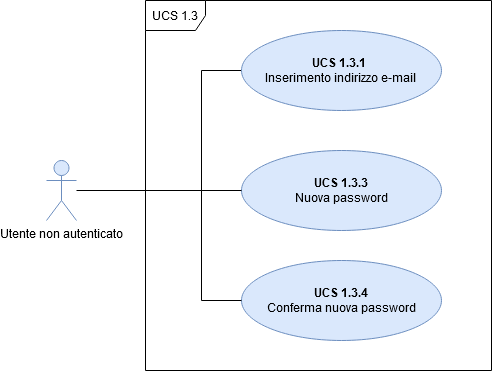
\includegraphics[scale=0.6]{Sezioni/UseCase/Immagini/UCS1.3.png}
	\caption{UCS 1.3 - Password dimenticata}
\end{figure}

\subsubsection{UCS 1.3 - Password dimenticata}%sea level
\begin{itemize}
\item \textbf{Attori primari:} Amministratore non autenticato
%\item \textbf{Attori secondari:}%opzionale
\item \textbf{Precondizione:}  L'amministratore non è autenticato.
\item \textbf{Postcondizione:} L'amministratore ha cambiato password con successo, la quale è stata salvata presso il sistema.
\item \textbf{Scenario principale:} L'amministratore non autenticato inserisce i dati necessari per cambiare la propria password.
\item \textbf{Flusso di eventi:}
    \begin{enumerate}
        \item Inserimento e-mail [UCS 1.3.1];
        \item E-mail cambio password [UCS 1.3.2];
        \item Nuova password [UCS 1.3.3];
        \item Conferma nuova password [UCS 1.3.4];
    \end{enumerate}
\end{itemize}

\subsubsection{UCS 1.3.1 - Inserimento e-mail}
\begin{itemize}
\item \textbf{Attori primari:} Amministratore non autenticato
\item \textbf{Precondizione:} L'amministratore non è autenticato. %è nella schermata di password dimenticata
\item \textbf{Postcondizione:} L'amministratore ha inserito l'e-mail.
\item \textbf{Scenario principale:} Inserimento dell'e-mail per cambiare la password.
\end{itemize}

\subsubsection{UCS 1.3.2 - E-mail cambio password}
\begin{itemize}
\item \textbf{Attori primari:} Amministratore non autenticato
\item \textbf{Precondizione:} L'amministratore non è autenticato.
\item \textbf{Postcondizione:} L'amministratore riceve l'email per il cambio password, ne consegue la necessità di reimpostare la password [UCS 1.3.3 e UCS 1.3.4].
\item \textbf{Scenario principale:} Ricevimento dell'e-mail per il cambio password.
\end{itemize}

\subsubsection{UCS 1.3.3 - Nuova password}
\begin{itemize}
\item \textbf{Attori primari:} Amministratore non autenticato
\item \textbf{Precondizione:}  L'amministratore non è autenticato.
\item \textbf{Postcondizione:} L'amministratore inserisce la nuova password.
\item \textbf{Scenario principale:} Inserimento della nuova password.
\end{itemize}

\subsubsection{UCS 1.3.4 - Conferma nuova password}
\begin{itemize}
\item \textbf{Attori primari:} Amministratore non autenticato
\item \textbf{Precondizione:} L'amministratore non è autenticato.
\item \textbf{Postcondizione:} L'amministratore reinserisce la nuova password per confermarla.
\item \textbf{Scenario principale:} Inserimento della conferma della nuova password.
\end{itemize}
